\chapter{A Precise Half-Wave Rectifier}


\section{Objectives}
\begin{itemize}
    \item To verify two precise half-wave rectifiers
\end{itemize}

\section{Materials}
\begin{itemize}
    \item Breadboard
    \item DC power supply
    \item Digital Multi-Meter
    \item \hyperref[1N4148]{Diode (1N4148)}
    \item Function Generator
    \item \hyperref[LM741_1]{Op.Amp. (LM741)}
    \item Oscilloscope
    \item Resistors
\end{itemize}

\section{Introduction}
    \subsection{Circuit Diagram}
    \begin{figure}[h]
    \centering
    \begin{subfigure}[h]{0.45\textwidth}
        \centering
        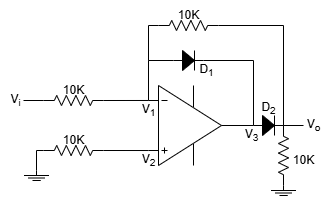
\includegraphics[width=0.7\linewidth]{Lab12/Lab12a.drawio.png}
        \caption{}
        \label{lab5a}
        \end{subfigure}
    \hfill
        \begin{subfigure}[h]{0.45\textwidth}
        \centering
        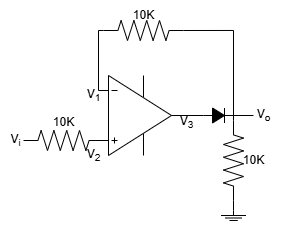
\includegraphics[width=0.7\linewidth]{Lab12/Lab12b.drawio.png}
        \caption{}
        \label{lab5b}
        \end{subfigure}
    \caption{Two precise half-wave rectifiers}
    \label{lab12f}
    \end{figure}
    \FloatBarrier

\section{Detailed Procedures}
    \subsection{Analyzation}


    \subsection{Procedures}

    
\section{Discussion}


\section{Conclusion}